\documentclass{article}

\usepackage{amsmath, enumerate, xcolor, tikz, pgfplots, array, bm, sfmath, tcolorbox, multicol}
\renewcommand{\familydefault}{\sfdefault}
\usepackage[top=0.5in, bottom=0.5in, left=1.25in, right=1.25in]{geometry}
\pagestyle{empty}
\raggedright

\pgfplotsset{compat = newest}
\usetikzlibrary{arrows.meta, calc, decorations.pathreplacing}
\pgfplotsset{every axis/.append style = {axis lines = middle}}
\pgfplotsset{every tick label/.append style={font=\scriptsize}}
\everymath{\displaystyle}

\newcounter{example}[section]
\newenvironment{example}[1][]{\refstepcounter{example}\par\medskip
   {\color{red}\textbf{Example~\theexample. #1}}}{\medskip}

\begin{document}

\section*{Limits}

\begin{tcolorbox}[colframe=orange!70!white, coltitle=black, title=\textbf{Summary}]
\begin{enumerate}
    \item The limit of a function as $x$ approaches a value is only concerned what happens as $x$ \emph{gets closer} to that value, not what happens \emph{at} that value.
    \item Limits can be found numerically, graphically, or algebraically.
\end{enumerate}
\end{tcolorbox}
\vspace{1in}

\subsection*{Limit Notation}

Consider $f(x) = \frac{x^2-4}{x-2}$. 
\begin{itemize}
    \item $f(2)$ is not defined (division by 0)
    \item What is the output behavior as $x$ \emph{gets closer} to 2?
\end{itemize}

We can fill out a table of values less than 2 and greater than 2:

\vfill 

\[
\lim_{x \to 2} \frac{x^2-4}{x-2} = 4
\]

\vspace{1in}

\newpage 

% As we increase the term numbers of a sequence such as
%     \[
%     1, \frac{1}{2}, \frac{1}{4}, \frac{1}{8}, \frac{1}{16}, \frac{1}{32}, \frac{1}{64}, \frac{1}{128}, \dots
%     \]
%     notice how the values of the terms get closer and closer to 0.   
% \vspace{0.5in}
    
% It {\color{red}\textbf{may or may not equal 0}} at some point, but we would say {\color{blue}\textbf{the limit of the sequence is 0.}}  \vspace{1.5in}


% Like sequences, functions can also have limits. \newline\\  
    
To indicate the limit $L$ of a function $f(x)$ as $x$ approaches the value of $a$, we use the notation
\[
\lim_{x \to a} f(x) = L
\]
\vspace{0.5in}

In other words, as $x$ gets closer to the $x$-coordinate $a$, \\ the $y$-values get closer to the $y$-coordinate $L$.  
\vspace{1in}

\begin{itemize}
    \item Sometimes you can just plug the value of $a$ into the function.
    \item Sometimes you can't (e.g. might get division by 0).
\end{itemize}
\vspace{1.5in}

\begin{center}
\fbox{\parbox{0.75\textwidth}{
\begin{center}
    {\color{red}\Large{\textbf{*** IMPORTANT ***}}} \newline\\
\end{center}


Limits only look at what happens {\color{blue}\textbf{as you get closer to the value of $\bm{a}$}}   \newline\\

They \textbf{are not concerned with} what the value of the function is \emph{at} that value of $a$.}}
\end{center}
\vfill 

\newpage

\begin{example}
Find each limit.
% \begin{multicols}{2}
\begin{enumerate}[(a)]
    \item $\lim_{x \to 7}\frac{x^2-6x-7}{x-7}$  \vfill 
    \item $\lim_{x \to 2}(3x+5)$
\end{enumerate}
% \end{multicols}
\end{example}

\vfill 



% \begin{example}
% Find $\lim_{x \to 5} \left(\frac{x^3-125}{x-5}\right)$  
% \end{example}
% \vfill 

% \begin{example}
% Find the limit. \emph{Note:} $x$ is in \underline{radians}.
%     \[
%     \lim_{x \to 0} \frac{\sin x}{x}
%     \]
% \end{example}


\subsection*{Left-Hand and Right-Hand Limits}

In the previous examples, we found limits by evaluating values less than the value of $a$ and also values greater than $a$. \newline\\
    
These are called {\color{blue}\textbf{left-hand limits}} and {\color{blue}\textbf{right-hand limits}}, respectively.
\vspace{1in}

\newpage 

\textsc{Left-Hand Limit}
    \[
    f(x) = \frac{x^2-6x-7}{x-7}
    \]
    \newline\\
    \begin{center}
    \begin{tabular}{c|c|c|c|c|}
        {} & \multicolumn{3}{|c|}{Values of $x$ approach 7 from the left ($x < 7$)} & \\ \hline
        $x$ & 6.99 & 6.999 & 6.9999 & 7 \\[6pt]
        $f(x)$ & \textbf{7.99} & \textbf{7.999} & \textbf{7.9999} & Undefined \\[8pt]
    \end{tabular}
    \end{center}
\vfill 

\textsc{Right-Hand Limit}
    \[
    f(x) = \frac{x^2-6x-7}{x-7}
    \]
    \newline\\
    \begin{center}
    \begin{tabular}{c|c|c|c|c|}
        {} & & \multicolumn{3}{|c|}{Values of $x$ approach 7 from the right ($x > 7$)} \\ \hline
        $x$ & 7 & 7.0001 & 7.001 & 7.01 \\[6pt]
        $f(x)$ & Undefined & \textbf{8.001} & \textbf{8.01} & \textbf{8.01} \\[8pt]
    \end{tabular}
    \end{center}
\vfill 

\begin{tabular}{cc}
        Left-Hand Limit: & $\lim_{x\to a^-} f(x)$ \\[18pt]
        Right-Hand Limit: & $\lim_{x\to a^+} f(x)$ \\
\end{tabular}

\vfill 

\textsc{Two-Sided Limit}
    \begin{center}
    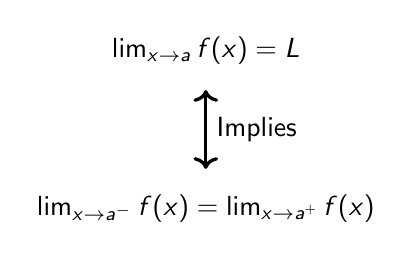
\begin{tikzpicture}
    \node at (0,0) {$\lim_{x \to a} f(x) = L$};
    \draw [<->, very thick] (0,-0.5) -- (0,-1.5) node [midway, right] {Implies};
    \node at (0,-2) {$\lim_{x \to a^-} f(x) = \lim_{x\to a^+} f(x)$};
    \end{tikzpicture}
    \end{center}
\vfill 
\newpage


\subsection*{Limits Using a Graph}

For $f(x)$ as $x$ approaches $a$:   
    \begin{itemize}
        \item Examine the graph to see if left-hand limit exists.  
        \begin{itemize}
            \item Won't if there is a vertical asymptote at $x=a$
        \end{itemize}
        \item Examine the graph to see if right-hand limit exists.
        \begin{itemize}
            \item Ditto from above
        \end{itemize}
        \item If the 2 one-sided limits exist and are equal, there is a ``limit."
        \item If there is a point at $x = a$, then $f(a)$ is the value of the function at $x=a$.
    \end{itemize}
\vfill 

\begin{example}
Use the graph of $f(x)$ to find each.   \newline\\
\begin{minipage}{0.45\textwidth}
    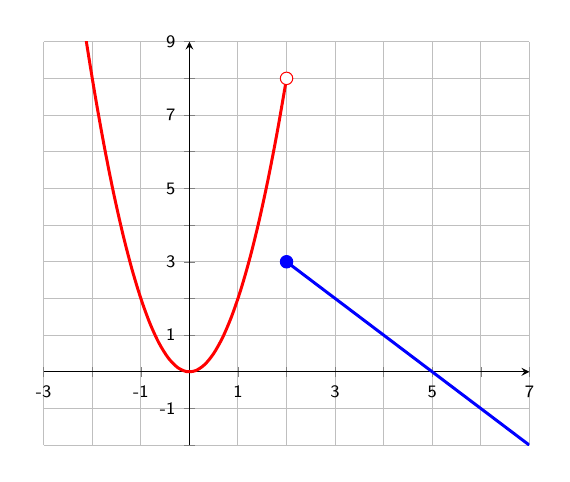
\begin{tikzpicture}[scale=0.9]
    \begin{axis}[
    xmin = -3, xmax =7,
    ymin = -2, ymax = 9,
    axis lines = middle,
    grid,
    xtick = {-3,-2,...,7},
    ytick = {-2,-1,...,9},
    xticklabels = {-3,,-1,,1,,3,,5,,7},
    yticklabels = {,-1,,1,,3,,5,,7,,9}
    ]
    \addplot[color=red,domain=-2.5:2,smooth,very thick] {2*x^2};
    \addplot[color=blue,domain=2:7,smooth,very thick] {5-x};
    \addplot[mark = *, mark size = 2.5pt, color=blue] coordinates {(2,3)};
    \addplot[mark = *, mark size = 2.5pt, color=red, fill=white] coordinates {(2,8)};
    \end{axis}
    \end{tikzpicture}
\end{minipage}
\hspace{-0.25cm}
\begin{minipage}{0.4\textwidth}
\begin{enumerate}[(a)] \setlength\itemsep{1cm}
    \item $\lim_{x\to 2^-} f(x)$
    \item $\lim_{x\to 2^+} f(x)$
    \item $\lim_{x\to 2} f(x)$
    \item $f(2)$
\end{enumerate}
\end{minipage}
\end{example}
\vfill 

\begin{example}
Use the graph of $f(x)$ to find each.   \newline\\
\begin{minipage}{0.45\textwidth}
    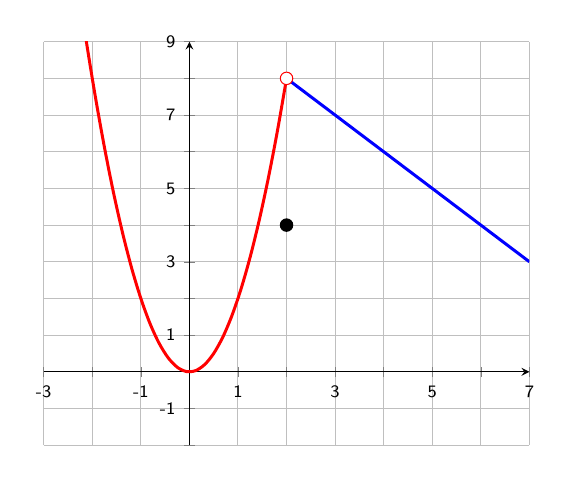
\begin{tikzpicture}[scale=0.9]
    \begin{axis}[
    xmin = -3, xmax =7,
    ymin = -2, ymax = 9,
    axis lines = middle,
    grid,
    xtick = {-3,-2,...,7},
    ytick = {-2,-1,...,9},
    xticklabels = {-3,,-1,,1,,3,,5,,7},
    yticklabels = {,-1,,1,,3,,5,,7,,9}
    ]
    \addplot[color=red,domain=-2.5:2,smooth,very thick] {2*x^2};
    \addplot[color=blue,domain=2:7,smooth,very thick] {10-x};
    \addplot[mark = *, mark size = 2.5pt] coordinates {(2,4)};
    \addplot[mark = *, mark size = 2.5pt, color=red, fill=white] coordinates {(2,8)};
    \end{axis}
    \end{tikzpicture}
\end{minipage}
\hspace{-0.25cm}
\begin{minipage}{0.4\textwidth}
\begin{enumerate}[(a)] \setlength\itemsep{1cm}
    \item $\lim_{x\to 2^-} f(x)$
    \item $\lim_{x\to 2^+} f(x)$
    \item $\lim_{x\to 2} f(x)$
    \item $f(2)$
\end{enumerate}
\end{minipage}  
\end{example}
\vfill 

\newpage 

% You can evaluate left- and right-hand limits of piecewise functions without needing to graph them. \newline\\

% As mentioned when we first discussed piecewise functions, pay attention to the domain for that piece of the function. \vspace{1in}

% \begin{example}
% Find each limit given the piecewise function below.

% \[
% f(x) = \begin{cases}
% 2\sin(x) + 1 & \text{if } x \leq -\pi \\[4pt] 
% x + \pi & \text{if } -\pi < x < 1 \\[4pt]
% 3.5 & \text{if } x = 1 \\[4pt]
% \log_5(x) + 2 & \text{if } 1 < x < 5 \\[4pt]
% -\sqrt{x-5} + 3 &\text{if } x \geq 5 \\[4pt]
% \end{cases}
% \]
% \smallskip 

% \begin{multicols}{4}
% \begin{enumerate}[(a)]
%     \item $\lim_{x \to -\pi^-} f(x)$
%     \item $\lim_{x \to -\pi^+} f(x)$
%     \item $\lim_{x \to -\pi} f(x)$
%     \item $f(-\pi)$
% \end{enumerate}
% \end{multicols}
% \vspace{0.75in}

% \begin{multicols}{4}
% \begin{enumerate}[(a)]  \setcounter{enumi}{4}
%     \item $\lim_{x \to 1^-} f(x)$
%     \item $\lim_{x \to 1^+} f(x)$
%     \item $\lim_{x \to 1} f(x)$
%     \item $f(1)$
% \end{enumerate}
% \end{multicols}
% \vspace{0.75in}

% \begin{multicols}{4}
% \begin{enumerate}[(a)]  \setcounter{enumi}{8}
%     \item $\lim_{x \to 5^-} f(x)$
%     \item $\lim_{x \to 5^+} f(x)$
%     \item $\lim_{x \to 5} f(x)$
%     \item $f(5)$
% \end{enumerate}
% \end{multicols}
% \end{example}

\subsection*{Algebraically Determining Limits}

\textsc{Limit Rules}: \newline\\

Let $a$, $c$, and $n$ be real numbers.
\begin{enumerate}
    \item $\lim_{x \to a} c = c$ (limit of a constant is that constant)
    \item $\lim_{x \to a} x = a$
    \item $\lim_{x \to a} \left[c \cdot f(x) \right] = c \cdot \lim_{x \to a} f(x)$
    \item $\lim_{x \to a} \left[f(x) \pm g(x)\right] = \lim_{x \to a} f(x) \pm \lim_{x \to a} g(x)$
    \item $\lim_{x \to a}\left[f(x) \cdot g(x)\right] = \lim_{x \to a} f(x) \cdot \lim_{x \to a} g(x)$
    \item $\lim_{x \to a} \frac{f(x)}{g(x)} = \frac{\lim_{x \to a} f(x)}{\lim_{x \to a} g(x)}$ provided $\lim_{x \to a} g(x) \neq 0$
    \item $\lim_{x \to a}\left[ f(x) \right]^n = \left[\lim_{x \to a} f(x) \right]^n$
\end{enumerate}
\vspace{1.5in}

\begin{example}
Determine each of the following limits.
\begin{multicols}{3}
\begin{enumerate}[(a)]
    \item $\lim_{x \to 2} 7$
    \item $\lim_{x \to 1} \left(2x^2 - 3x + 5\right)$
    \item $\lim_{x \to 3} \sqrt{2x-1}$
\end{enumerate}
\end{multicols}
\end{example}

\newpage 

You can also use techniques like factoring before evaluating limits.

\begin{example}
Find each limit algebraically.
\begin{multicols}{2}
\begin{enumerate}[(a)]
    \item $\lim_{x \to 7} \frac{x^2-6x-7}{x-7}$
    \item $\lim_{x \to 3} \frac{x^2-9}{x-3}$
\end{enumerate}
\end{multicols}
\end{example}
\vfill 

When two variables are involved, keep in mind {\color{blue}\textbf{which variable}} is changing in the limit.

\begin{example}
Find each limit.
\begin{multicols}{2}
\begin{enumerate}[(a)]
    \item $\lim_{h \to 0}\left(3x + 2h\right)$
    \item $\lim_{h \to 0}\frac{5xh+2h^2}{h}$
\end{enumerate}
\end{multicols}
\end{example}
\vfill 

\newpage 

\begin{example}
For $f(x) = x^2$, compute $\lim_{h \to 0} \frac{f(2+h)-f(2)}{h}$
\end{example}

\end{document}
